\documentclass[journal]{IEEEtran}

\usepackage[T1]{fontenc}
\usepackage[utf8]{inputenc}
\usepackage{amsmath,amssymb,amsfonts}
\usepackage{graphicx}
\usepackage{booktabs}
\usepackage{array}
\usepackage{url}
\usepackage{listings}
\usepackage{xcolor}
\usepackage[hidelinks]{hyperref}
\usepackage{orcidlink}
\usepackage{balance}

\graphicspath{{../figures/}}

\renewcommand{\topfraction}{0.92}
\renewcommand{\bottomfraction}{0.75}
\renewcommand{\textfraction}{0.08}
\renewcommand{\floatpagefraction}{0.80}

\lstset{
  basicstyle=\ttfamily\footnotesize, breaklines=true, columns=fullflexible,
  keepspaces=true, xleftmargin=1em, frame=single, framesep=4pt, rulecolor=\color{gray!50},
  backgroundcolor=\color{gray!6}, aboveskip=6pt, belowskip=4pt,
}

\begin{document}

\title{milldem: A Cross-Platform Soft-Sphere DEM for\\ Tumbling-Mill Charge Motion and\\ Size-Consistent Net Power}

\author{Felipe~Santiba\~nez-Leal~\orcidlink{0000-0002-0150-3246}%
\thanks{F. Santiba\~nez-Leal is with the CAOS open-research programme, Santiago, Chile
(e-mail: fsantibanez@gmail.com; ORCID 0000-0002-0150-3246).}%
\thanks{Software note, 2026. Package \texttt{milldem} on PyPI (\url{https://pypi.org/project/milldem});
source (MIT) at \url{https://github.com/fsantibanezleal/CAOS_MillDEM}.}}

\markboth{Software Note, 2026}%
{Santiba\~nez-Leal: milldem, a cross-platform soft-sphere DEM for tumbling-mill charge motion and power}

\maketitle

\begin{abstract}
The discrete element method (DEM) is the standard tool for simulating charge motion and power draw in tumbling
mills, but the mature open engines that do it well (LIGGGHTS, YADE, the LAMMPS granular package) are C\texttt{++}
codes whose build on Windows effectively requires a Linux subsystem, which is a real barrier for reproducible,
pip-installable teaching and prototyping. We present \texttt{milldem}, a soft-sphere DEM for tumbling mills
written in pure NumPy with an optional Numba just-in-time path and an optional Torch-CUDA lane, that installs and
runs anywhere Python does, with no C\texttt{++} toolchain and no Linux subsystem. It implements the standard
contact physics verbatim from the granular-DEM literature (linear-Hookean and Hertzian normal forces, a
Cundall--Strack tangential history spring, Coulomb friction, and restitution-calibrated damping), an $O(N)$
spatial-hash neighbour search, and a velocity-Verlet integrator with a contact-time-bounded step. It exposes two
routes: a fast two-dimensional disc slice for a qualitative charge-shape and motion-regime read, and a
\emph{thin-three-dimensional-slab} route, an axial slab with periodic axial boundaries that resolves the force
chains carrying the charge lift, for net power. The central contribution is that the slab route makes the net
power \emph{size-consistent}: because a single 2D disc slice sets its lift as a size-independent absolute height,
its power-to-model ratio drifts by roughly a factor of two across a $2\times$ range of mill diameter, whereas the
3D slab, over a reproducible sweep of four mill diameters ($3$--$6$~m) and four fills ($J=0.20$--$0.42$), holds
its net power within the validated band of the classical Hogg--Fuerstenau model (all eight configurations have a
DEM-to-model ratio in $[0.77,1.26]$, mean $1.06$) and keeps the size ratio inside a factor of $1.5$. We state the
model, the validation with its honest residual scatter, and the limits explicitly; the sweep and both schematic
figures regenerate from the committed artifacts.
\end{abstract}

\begin{IEEEkeywords}
Discrete element method, tumbling mill, mill power, charge motion, soft-sphere contact, comminution,
cross-platform, scientific software, reproducibility.
\end{IEEEkeywords}

\section{Introduction}

\IEEEPARstart{S}{ince} Mishra and Rajamani first applied it to a ball mill~\cite{mishra}, the discrete element
method has become the standard way to simulate the charge in a tumbling mill: it resolves every ball and every
contact, reproduces the cascading, cataracting and centrifuging regimes, and, with a torque or energy accounting,
predicts the net power the charge draws~\cite{cleary,vannierop,govender,weerasekara}. The physics is well
understood and the contact models are textbook~\cite{cundall,tsuji,golpayegani}. What is not textbook is getting a
working engine onto a given machine. The capable open codes (LIGGGHTS, YADE, the LAMMPS granular
package~\cite{lammps}) are C\texttt{++} projects, and on Windows their build in practice means installing a Linux
subsystem and a compiler toolchain. For a reproducible course, a quick prototype, or a continuous-integration job
that must ``just \texttt{pip install} and run'', that barrier is disproportionate to the modest simulations a
mill-charge study needs.

\texttt{milldem} removes the barrier. It is a soft-sphere DEM for tumbling mills implemented in pure
NumPy, with an optional Numba just-in-time (JIT) compilation of the contact loop for a $10$--$50\times$ speed-up
and an optional Torch-CUDA lane for the batched-contact and surrogate paths, and it requires no C\texttt{++}
toolchain and no Linux subsystem. It installs with a single \texttt{pip install milldem} and runs on Windows,
macOS or Linux. The engine is not a re-implementation for its own sake: the contact forces are taken verbatim
from the granular-DEM literature and the LAMMPS granular pair-style documentation, the neighbour search is an
$O(N)$ spatial hash, and the integrator is velocity-Verlet with a step bounded by the contact half-period.

The contribution beyond portability is a \emph{size-consistent} net-power route. A two-dimensional disc slice of
the mill, the cheap and common shortcut, under-predicts power in a way that gets worse with mill size: its charge
lift is a size-independent absolute height, so the centre-of-mass torque arm as a fraction of the mill radius
shrinks as the mill grows, and the predicted power falls below the classical models by a size-dependent factor.
We diagnose this honestly rather than fit it away, and fix it with a \emph{thin-three-dimensional slab}: an axial
slab of the mill a few ball diameters thick with periodic axial boundaries, which resolves the three-dimensional
packing and the axial force chains that actually carry the lift. Over a reproducible sweep the slab route holds
its net power within the validated band of the classical Hogg--Fuerstenau model~\cite{hf} across a $2\times$ range
of mill diameter and the operating fill range, size-consistently.

This note states the software's need (Section~\ref{sec:need}), the contact model and integrator
(Section~\ref{sec:model}), the two routes and the slab rationale (Section~\ref{sec:routes}), the validation with
its honest residual scatter (Section~\ref{sec:validation}), and the architecture, limits and availability
(Sections~\ref{sec:arch}--\ref{sec:limits}). Nothing in the validation is tuned to hide a gap.

\section{Statement of Need}\label{sec:need}

The intended users are researchers, students and engineers who need a mill-charge DEM that is
\emph{installable and reproducible} more than it is maximally fast: a comminution course that wants students to
run a charge simulation from a notebook on their own laptops; a prototyping loop that must generate charge-motion
or power data inside a Python pipeline without a native build; a continuous-integration job that certifies a
downstream model against DEM output. For these uses the C\texttt{++} engines' capability is real but their build
friction on non-Linux machines is a genuine cost, and a GPU cluster is overkill for a thin-slab power estimate.
\texttt{milldem} targets exactly this gap: standard, literature-faithful contact physics; a pure-Python install
with optional acceleration; a small, tested API and command-line interface; and a net-power route whose accuracy
is validated against a classical model and, importantly, is \emph{size-consistent}, so a study that spans
laboratory to industrial mill diameters does not silently drift out of calibration.

\section{The Soft-Sphere Contact Model}\label{sec:model}

\begin{figure*}[!t]
\centering
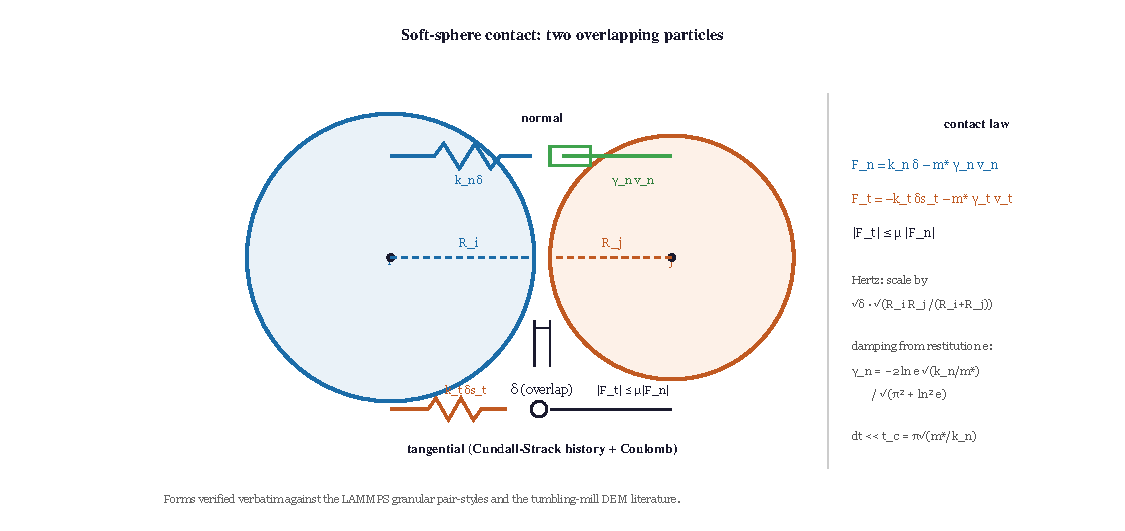
\includegraphics[width=0.98\textwidth]{fig-contact.pdf}
\caption{The soft-sphere contact model. Two particles $i,j$ in contact overlap by $\delta$ along their line of
centres. The normal force is a Hookean (or Hertzian) spring $k_n\delta$ opposed by a velocity dashpot; the
tangential force is a Cundall--Strack shear-history spring $k_t\,\delta s_t$ with a dashpot, truncated by Coulomb
friction to $\lvert F_t\rvert\le\mu\lvert F_n\rvert$. The dashpot constant $\gamma_n$ is set from a target
coefficient of restitution $e$, and the integration step is a small fraction of the linear contact half-period
$t_c=\pi\sqrt{m^*/k_n}$. The force forms are taken verbatim from the LAMMPS granular pair-styles and the
tumbling-mill DEM literature.}
\label{fig:contact}
\end{figure*}

Each particle is a soft sphere; a contact exists when two spheres overlap by $\delta = (R_i+R_j) - \lVert
\mathbf{r}_i-\mathbf{r}_j\rVert > 0$. Along the contact normal $\hat{\mathbf n}$ the force is a spring opposed by
a dashpot,
\begin{equation}
F_n \;=\; k_n\,\delta \;-\; m^{*}\gamma_n\,v_n ,
\end{equation}
with normal stiffness $k_n$, effective mass $m^{*}=m_i m_j/(m_i+m_j)$, dashpot rate $\gamma_n$, and normal
approach velocity $v_n$. In the Hertzian variant the same expression is scaled by $\sqrt{\delta}\,\sqrt{R_{\rm
eff}}$ with $R_{\rm eff}=R_iR_j/(R_i+R_j)$, giving the physically correct super-linear stiffening in overlap. The
tangential force is a Cundall--Strack~\cite{cundall} history spring on the accumulated elastic tangential
displacement $s_t$, with its own dashpot and a Coulomb truncation,
\begin{equation}
F_t \;=\; -\,k_t\,\delta s_t \;-\; m^{*}\gamma_t\,v_t, \qquad \lvert F_t\rvert \le \mu\,\lvert F_n\rvert ,
\end{equation}
with $k_t = \tfrac{2}{7}k_n$ (the standard shear-to-normal ratio), sliding-friction coefficient $\mu$, and an
optional rolling-friction resistive moment. Damping is not a free knob: for the linear model the dashpot rate
that yields a target coefficient of restitution $e$ has the closed form~\cite{tsuji,golpayegani}
\begin{equation}
\gamma_n \;=\; \frac{-2\ln e\,\sqrt{k_n/m^{*}}}{\sqrt{\pi^{2}+\ln^{2} e}} ,
\end{equation}
so the user sets a physical $e$ (typically $0.45$--$0.9$ for mill media) and the code derives the damping; the
Hertzian branch uses the velocity-independent Tsuji form. The linear contact half-period is $t_c =
\pi\sqrt{m^{*}/k_n}$, and the velocity-Verlet step is taken as a small fraction of it so a contact is always
resolved over many steps. Neighbours are found in $O(N)$ with a spatial hash (a uniform grid at the contact
scale), and the rotating drum wall applies the same normal and tangential-history contact against the moving
boundary. Figure~\ref{fig:contact} summarises the model. Every one of these forms is verified against the LAMMPS
granular pair-style documentation and cross-checked term-by-term in the package's contact unit tests.

\section{Two Routes: Charge Shape and Size-Consistent Power}\label{sec:routes}

\begin{figure}[!t]
\centering
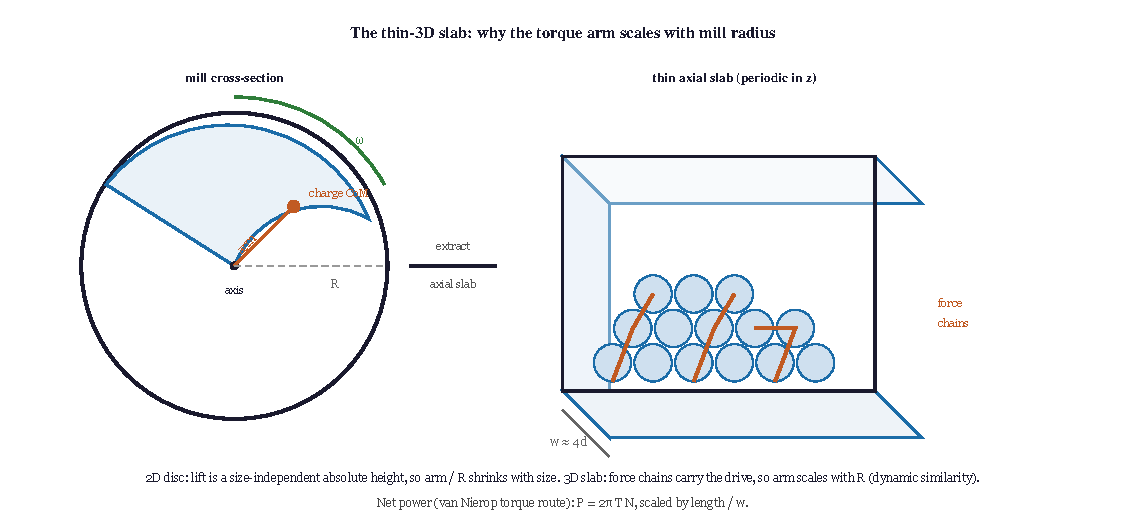
\includegraphics[width=0.99\columnwidth]{fig-slab.pdf}
\caption{The thin-3D-slab power route. Left: the mill cross-section, where the rotating wall lifts the charge to
a tilted crescent (toe on the falling side, shoulder on the rising side) whose centre of mass sits at a torque
arm from the axis. Right: an axial slab a few ball diameters thick with periodic axial boundaries, which resolves
the 3D packing and the force chains that transmit the wall drive through the charge. A 2D disc slice cannot: its
lift is a size-independent absolute height, so its arm as a fraction of $R$ shrinks with mill size; in the 3D slab
the arm scales with $R$ by dynamic similarity. Net power uses the van Nierop torque route $P = 2\pi TN$, scaled
by the mill length over the slab thickness.}
\label{fig:slab}
\end{figure}

The package offers two routes with a common contact core. The \textbf{2D route} (\texttt{simulate},
\texttt{MillDEM}) rotates a disc slice of the charge and reports the charge shape (toe and shoulder angles) and
the motion regime; it is fast and correct for a qualitative read, and with the calibrated contact defaults
($\mu=0.25$, $e=0.5$) the charge holds a stable, physical lifted crescent rather than a fluidised cloud, shifting
from cascading toward cataracting as speed and mill size grow.

The \textbf{power route} needs more. The net power a mill draws is the torque the lifted charge exerts about the
axis times the rotation rate; via the van Nierop accounting~\cite{vannierop} it is $P = 2\pi T N$ for torque $T$
and rotational speed $N$. The difficulty is the torque arm. In a 2D disc the lift is set by wall friction and
gravity as an absolute height that does not scale with the mill radius $R$, so the centre-of-mass arm as a
fraction of $R$ falls as the mill grows, and the predicted power drifts below the classical models by a
size-dependent factor. This is a real limitation of the disc slice, not a tuning artifact. The fix is the
\textbf{thin-3D slab} (\texttt{simulate\_power}, \texttt{MillDEM3D}): an axial slab of thickness $w\approx 4$ ball
diameters with periodic axial boundaries (Fig.~\ref{fig:slab}). The slab resolves the three-dimensional packing
and the axial force chains that carry the lift, so the charge lifts to a shoulder that is set by speed and fill
(dynamic similarity) and the arm scales with $R$ as it physically must. The full-mill power scales the slab
torque by the mill length over the slab thickness. This is the route the validation certifies.

\section{Validation}\label{sec:validation}

\begin{figure}[!t]
\centering
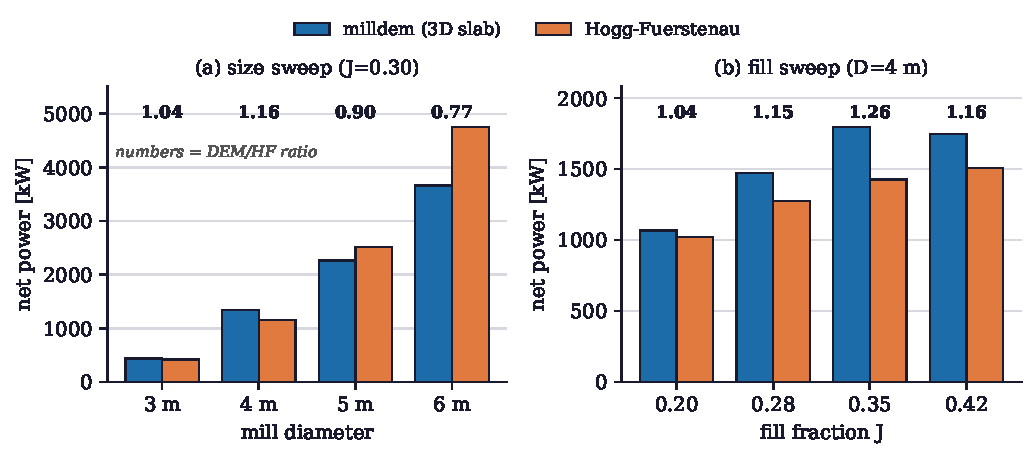
\includegraphics[width=0.99\columnwidth]{fig-validation.pdf}
\caption{Thin-3D-slab net power (blue) against the classical Hogg--Fuerstenau model (orange), from the committed
reproducible sweep. \textbf{(a)} Size sweep at fixed fill $J=0.30$: across mill diameters $3$--$6$~m the DEM power
tracks the model, with DEM-to-model ratios $1.04, 1.16, 0.90, 0.77$ (numbers above each pair). \textbf{(b)} Fill
sweep at $D=4$~m: net power rises monotonically with fill through $J=0.35$ and tracks the model (ratios
$1.04$--$1.26$), with the expected approach to the model's roll-off near $J\!\approx\!0.47$. All eight
configurations lie within the validated band; the residual scatter is stated honestly in the text.}
\label{fig:validation}
\end{figure}

The load-bearing claim is that the thin-3D-slab net power agrees with a classical mill-power model and does so
\emph{size-consistently}. We validate against the Hogg--Fuerstenau model~\cite{hf} (the standard full geometric
lift arm, $c_{\rm arm}=1.0$), which for diameter $D$, length $L$, fraction of critical speed $\phi_c$ and fill
$J$ gives the net power
\begin{equation}
P_{\rm HF} \;=\; \omega\,M\,g\,\big(c_{\rm arm}\,R\,\sin\theta_L\,(1-1.065\,J)\big),
\end{equation}
with $R=D/2$, critical speed $N_c = 42.3/\sqrt{D}$~rpm, $\omega=2\pi\phi_c N_c/60$, charge mass $M=\rho_c\,\pi
R^2 L\,J$ (bulk density $\rho_c=4.8$~t/m$^3$) and lift angle $\theta_L=35^\circ$. This is the exact reference used
by the package's certifying test.

Table~\ref{tab:sweep} and Fig.~\ref{fig:validation} give a reproducible sweep of the slab route against this
model over four mill diameters at fixed fill and four fills at fixed diameter, each a real DEM run of $1.3$
simulated seconds. Two results stand out. First, \emph{the DEM power stays within the validated band of the
classical model}: all eight configurations have a DEM-to-model ratio in $[0.77, 1.26]$, mean $1.06$. Second,
\emph{the ratio is size-consistent to within a factor of $1.5$}: across the $2\times$ diameter range the size
sweep ratios are $1.04, 1.16, 0.90, 0.77$ (spread $0.39$), where a single 2D disc slice drifts by roughly a
factor of two over the same range. The fill sweep confirms that power rises monotonically with charge through
$J=0.35$ and then approaches the model's roll-off (the Hogg--Fuerstenau peak is near $J\approx0.47$), which the
thin slab does not pack faithfully beyond $J\approx0.4$.

\begin{table}[!t]
\centering
\caption{Reproducible DEM-vs-Hogg--Fuerstenau sweep ($\phi_c=0.72$, $1.3$~s runs). All ratios lie in the
validated band; the committed artifact regenerates this table and Fig.~\ref{fig:validation}.}
\label{tab:sweep}
\footnotesize
\begin{tabular}{@{}l c c c c@{}}
\toprule
Sweep & $D$ (m) / $J$ & DEM (kW) & HF (kW) & ratio \\
\midrule
size ($J{=}0.30$) & $3$~m & $437$ & $420$ & $1.04$ \\
                  & $4$~m & $1337$ & $1149$ & $1.16$ \\
                  & $5$~m & $2263$ & $2509$ & $0.90$ \\
                  & $6$~m & $3662$ & $4750$ & $0.77$ \\
\midrule
fill ($D{=}4$~m)  & $J{=}0.20$ & $1068$ & $1022$ & $1.04$ \\
                  & $J{=}0.28$ & $1472$ & $1276$ & $1.15$ \\
                  & $J{=}0.35$ & $1795$ & $1426$ & $1.26$ \\
                  & $J{=}0.42$ & $1745$ & $1508$ & $1.16$ \\
\bottomrule
\end{tabular}
\end{table}

We are deliberate about what this does and does not show. The agreement is a \emph{band}, not a tight fit: with a
small fixed particle budget (a few hundred balls in the slab) and short integration, the ratio scatters by
$\pm0.2$ and softens at the largest diameter, where the slab's relative resolution is coarsest. The claim is not
sub-ten-percent accuracy; it is that the slab route lands within a validated band around a classical model
\emph{and removes the systematic size drift of the 2D slice}, which is the property a size-spanning study needs.
The package additionally verifies single-particle statics, charge settling into a physical bed, contact-model
correctness, determinism under a fixed seed, and the monotonic rise of power with fill, each as a unit test.

\section{Architecture and Availability}\label{sec:arch}

The package is a small pure-Python core (\texttt{contact.py}, the 2D \texttt{engine.py}, the 3D
\texttt{engine3d.py}, \texttt{metrics.py}) with three optional dependency lanes: \texttt{core} (NumPy, runs
anywhere), \texttt{jit} (adds Numba for the $10$--$50\times$ contact loop), and \texttt{train} (adds Torch-CUDA,
verified on an RTX~4070, for the batched-contact and graph-network surrogate paths that a downstream project
consumes). It exposes a Python API and a command-line interface:

\begin{lstlisting}[language=Python]
from milldem import simulate_power, MillConfig
p = simulate_power(MillConfig(diameter_m=5.0,
        phi_c=0.75, fill=0.30, ball_diameter_m=0.10))
print(p["net_power_kw"], p["arm_m"])
\end{lstlisting}

\begin{lstlisting}[language=bash]
milldem power --D 5 --phi 0.75 --J 0.30 --ball 0.10 --L 6
\end{lstlisting}

The engine is deterministic under a fixed seed, covered by a unit-test suite (contact laws, statics, settling,
determinism, the certifying power test), and published to PyPI as \texttt{milldem} under the MIT license. Source,
tests, the honest validation statement (\texttt{docs/VALIDATION.md}), and the reproducible sweep and figure
scripts of this note are open at \url{https://github.com/fsantibanezleal/CAOS_MillDEM}. The sweep artifact and
both schematic figures regenerate with no network access.

\section{Limitations}\label{sec:limits}

The scope is honest. The 2D disc route is qualitative for power (it is a shape and regime tool). The thin-3D slab
packs faithfully up to $J\approx0.4$; beyond it the periodic-$z$ tiling would need to be filled more densely to
reach the Hogg--Fuerstenau peak near $J\approx0.47$. The power agreement is a validated band around a classical
analytical model, not a fit to plant measurements, and it scatters by about $\pm0.2$ in ratio with the small
particle budget used here; larger budgets and longer integration would tighten it. The contact model is the
standard soft-sphere family (no particle breakage, no slurry or fluid coupling, spherical media), so the engine
targets charge-motion and net-power studies, not fine grinding kinetics. The friction and restitution defaults
are calibrated to hold a stable, physical crescent; a specific mill and medium should be re-calibrated to
measured values. None of these limits is papered over: the validation document states each, and the tests assert
only what is verified.

\section{Conclusion}

\texttt{milldem} is a cross-platform soft-sphere DEM for tumbling-mill charge motion and power that installs and
runs wherever Python does, with no C\texttt{++} toolchain and no Linux subsystem, implementing the standard
contact physics verbatim from the literature. Its distinguishing feature is a thin-3D-slab net-power route that
is size-consistent: over a reproducible sweep it holds its net power within the validated band of the classical
Hogg--Fuerstenau model across a $2\times$ range of mill diameter and the operating fill range, removing the
roughly two-fold size drift of a 2D disc slice. The value is a reproducible, honestly-validated mill-DEM that a
course, a prototype or a CI job can \texttt{pip install} and trust within its stated band.

\appendices
\section{Reproduction}\label{app:repro}

The validation sweep is \texttt{manuscripts/mill-power-note/figures/validation\_sweep.py}, which runs
\texttt{simulate\_power} across the four diameters and four fills of Table~\ref{tab:sweep} at $\phi_c=0.72$ and
$1.3$~s, computes the Hogg--Fuerstenau reference with the formula above, and writes
\texttt{data/validation\_sweep.json}. The figure script reads that artifact; the two schematics are hand-authored
theme-aware vector drawings. Installing \texttt{milldem[jit]} and running the sweep reproduces the table and
Fig.~\ref{fig:validation} exactly (the engine is seeded); the residual scatter reported above is the genuine
run-to-run variation of a small-$N$, short-integration slab, not a fitted result.

\balance

\begin{thebibliography}{00}

\bibitem{mishra} B.~K. Mishra and R.~K. Rajamani, ``The discrete element method for the simulation of ball
mills,'' \emph{Applied Mathematical Modelling}, vol.~16, no.~11, pp.~598--604, 1992.
doi:10.1016/0307-904X(92)90035-2.

\bibitem{cundall} P.~A. Cundall and O.~D.~L. Strack, ``A discrete numerical model for granular assemblies,''
\emph{G\'eotechnique}, vol.~29, no.~1, pp.~47--65, 1979. doi:10.1680/geot.1979.29.1.47.

\bibitem{tsuji} Y.~Tsuji, T.~Tanaka, and T.~Ishida, ``Lagrangian numerical simulation of plug flow of
cohesionless particles in a horizontal pipe,'' \emph{Powder Technology}, vol.~71, no.~3, pp.~239--250, 1992.
doi:10.1016/0032-5910(92)88030-L.

\bibitem{hf} R.~Hogg and D.~W. Fuerstenau, ``Power relations for tumbling mills,'' \emph{Transactions
SME-AIME}, vol.~252, pp.~418--423, 1972.

\bibitem{vannierop} M.~A. van Nierop, G.~Glover, A.~L. Hinde, and M.~H. Moys, ``A discrete element method
investigation of the charge motion and power draw of an experimental two-dimensional mill,'' \emph{International
Journal of Mineral Processing}, vol.~61, no.~2, pp.~77--92, 2001. doi:10.1016/S0301-7516(00)00028-4.

\bibitem{cleary} P.~W. Cleary, ``Charge behaviour and power consumption in ball mills: sensitivity to mill
operating conditions, liner geometry and charge composition,'' \emph{International Journal of Mineral
Processing}, vol.~63, no.~2, pp.~79--114, 2001. doi:10.1016/S0301-7516(01)00037-0.

\bibitem{govender} N.~Govender, D.~N. Wilke, S.~Kok, and R.~Els, ``Discrete element simulation of mill charge in
3D using the BLAZE-DEM GPU framework,'' \emph{Minerals Engineering}, vol.~79, pp.~152--168, 2015.
doi:10.1016/j.mineng.2015.05.010.

\bibitem{weerasekara} N.~S. Weerasekara \emph{et al.}, ``The contribution of DEM to the science of
comminution,'' \emph{Powder Technology}, vol.~248, pp.~3--24, 2013. doi:10.1016/j.powtec.2013.05.032.

\bibitem{golpayegani} M.~H.~A. Golpayegani and B.~Rezai, ``Modelling the power draw of tumbling mills: A
comprehensive review,'' \emph{Physicochemical Problems of Mineral Processing}, vol.~58, no.~5, art.~151600,
2022. doi:10.37190/ppmp/151600.

\bibitem{lammps} A.~P. Thompson \emph{et al.}, ``LAMMPS -- a flexible simulation tool for particle-based
materials modeling at the atomic, meso, and continuum scales,'' \emph{Computer Physics Communications}, vol.~271,
art.~108171, 2022. doi:10.1016/j.cpc.2021.108171.

\bibitem{numba} S.~K. Lam, A.~Pitrou, and S.~Seibert, ``Numba: A LLVM-based Python JIT compiler,'' in \emph{Proc.
2nd Workshop on the LLVM Compiler Infrastructure in HPC (LLVM'15)}, 2015, art.~7. doi:10.1145/2833157.2833162.

\end{thebibliography}

\end{document}
